\begin{surferPage}[Ettagono]{Una Settica ettagono-simmetrica}
    Questa superficie dalle sembianze di una stella ha grado $7$. Fino a poco tempo fa, il numero delle sue singolarit\`a ($84$) era ancora il massimo numero conosciuto di singolarit\`a reali per le settiche (superfici di grado $7$); solo nel 2004 Oliver Labs miglior\`o questo record mondiale portandolo a $99$.
      
    I tre cuscini che si possono vedere nella figura interattiva sono dovuti all'uso dei polinomi di Tchebychev, analogamente a quanto accade per l'Ottica di Chmutov. 
    In effetti, questa superficie a forma di stella \`e un'altra variante delle superfici di Chmutov.
    Qui la curva piana di equazione $T_d(x)+T_d(y)=0$ \`e stata sostituita da un ettagono (poligono con $7$ lati e $7$ angoli) regolare $S_7(x,y)$: 
   \[S_7(x,y) + \lambda \cdot T_d(z) = 0,\]
    per un numero reale $\lambda$ opportunamente scelto. 
    \vspace*{-0.3em}
    \begin{center}
      \begin{tabular}{c@{\qquad}c}
        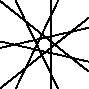
\includegraphics[height=1.5cm]{./../../common/images/labsseptic1.pdf}
        &
        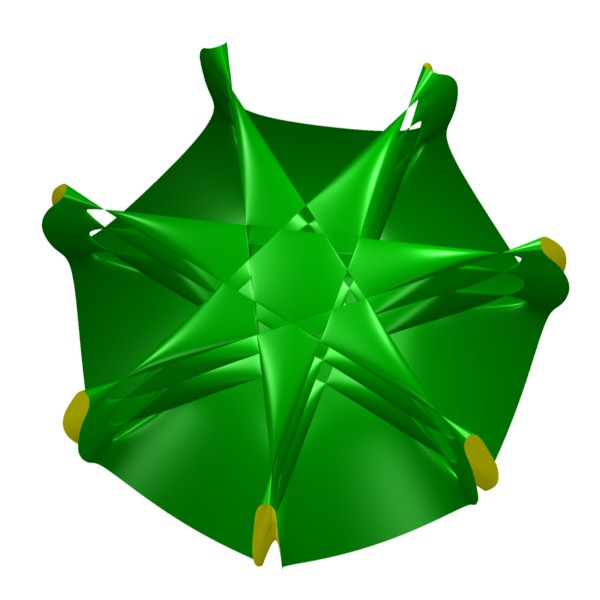
\includegraphics[height=1.5cm]{./../../common/images/septic_7eck_von_oben}
      \end{tabular}
    \end{center}
    \vspace*{-0.3em}   
   Questa variante della costruzione di Chmutov \`e dovuta a Duco van Straten.
\end{surferPage}
